% This template has been tested with LLNCS DOCUMENT CLASS -- version 2.20 (10-Mar-2018)

% !TeX spellcheck = en-US
% !TeX encoding = utf8
% !TeX program = pdflatex
% !BIB program = bibtex
% -*- coding:utf-8 mod:LaTeX -*-

% "a4paper" enables:
%  - easy print out on DIN A4 paper size
%
% One can configure a4 vs. letter in the LaTeX installation. So it is configuration dependend, what the paper size will be.
% This option  present, because the current word template offered by Springer is DIN A4.
% We accept that DIN A4 cause WTFs at persons not used to A4 in USA.

% "runningheads" enables:
%  - page number on page 2 onwards
%  - title/authors on even/odd pages
% This is good for other readers to enable proper archiving among other papers and pointing to
% content. Even if the title page states the title, when printed and stored in a folder, when
% blindly opening the folder, one could hit not the title page, but an arbitrary page. Therefore,
% it is good to have title printed on the pages, too.
%
% It is enabled by default as the springer template as of 2018/03/10 uses this as default

% German documents: pass ngerman as class option
 \documentclass[ngerman,runningheads,a4paper]{llncs}[2018/03/10]
% English documents: pass english as class option
%\documentclass[english,runningheads,a4paper]{llncs}[2018/03/10]

%% If you need packages for other papers,
%% START COPYING HERE

% Set English as language and allow to write hyphenated"=words
%
% In case you write German, switch the parameters, so that the command becomes
\usepackage[english,main=ngerman]{babel}
%
% Even though `american`, `english` and `USenglish` are synonyms for babel package (according to https://tex.stackexchange.com/questions/12775/babel-english-american-usenglish), the llncs document class is prepared to avoid the overriding of certain names (such as "Abstract." -> "Abstract" or "Fig." -> "Figure") when using `english`, but not when using the other 2.
% english has to go last to set it as default language
%\usepackage[ngerman,main=english]{babel}
%
% Hint by http://tex.stackexchange.com/a/321066/9075 -> enable "= as dashes
\addto\extrasenglish{\languageshorthands{ngerman}\useshorthands{"}}
%
% Fix by https://tex.stackexchange.com/a/441701/9075
\usepackage{regexpatch}
\makeatletter
\edef\switcht@albion{%
  \relax\unexpanded\expandafter{\switcht@albion}%
}
\xpatchcmd*{\switcht@albion}{ \def}{\def}{}{}
\xpatchcmd{\switcht@albion}{\relax}{}{}{}
\edef\switcht@deutsch{%
  \relax\unexpanded\expandafter{\switcht@deutsch}%
}
\xpatchcmd*{\switcht@deutsch}{ \def}{\def}{}{}
\xpatchcmd{\switcht@deutsch}{\relax}{}{}{}
\edef\switcht@francais{%
  \relax\unexpanded\expandafter{\switcht@francais}%
}
\xpatchcmd*{\switcht@francais}{ \def}{\def}{}{}
\xpatchcmd{\switcht@francais}{\relax}{}{}{}
\makeatother

\usepackage{ifluatex}
\ifluatex
  \usepackage{fontspec}
  \usepackage[english]{selnolig}
\fi

\iftrue % use default-font
  \ifluatex
    % use the better (sharper, ...) Latin Modern variant of Computer Modern
    \setmainfont{Latin Modern Roman}
    \setsansfont{Latin Modern Sans}
    \setmonofont{Latin Modern Mono} % "variable=false"
    %\setmonofont{Latin Modern Mono Prop} % "variable=true"
  \else
    % better font, similar to the default springer font
    % cfr-lm is preferred over lmodern. Reasoning at http://tex.stackexchange.com/a/247543/9075
    \usepackage[%
      rm={oldstyle=false,proportional=true},%
      sf={oldstyle=false,proportional=true},%
      tt={oldstyle=false,proportional=true,variable=false},%
      qt=false%
    ]{cfr-lm}
  \fi
\else
  % In case more space is needed, it is accepted to use Times New Roman
  \ifluatex
    \setmainfont{TeX Gyre Termes}
    \setsansfont[Scale=.9]{TeX Gyre Heros}
    % newtxtt looks good with times, but no equivalent for lualatex found,
    % therefore tried to replace with inconsolata.
    % However, inconsolata does not look good in the context of LNCS ...
    %\setmonofont[StylisticSet={1,3},Scale=.9]{inconsolata}
    % ... thus, we use the good old Latin Modern Mono font for source code.
    \setmonofont{Latin Modern Mono} % "variable=false"
    %\setmonofont{Latin Modern Mono Prop} % "variable=true"
  \else
    % overwrite cmodern with the Times variant
    \usepackage{newtxtext}
    \usepackage{newtxmath}
    \usepackage[zerostyle=b,scaled=.9]{newtxtt}
  \fi
\fi

\ifluatex
\else
  % fontenc and inputenc are not required when using lualatex
  \usepackage[T1]{fontenc}
  \usepackage[utf8]{inputenc} %support umlauts in the input
\fi

\usepackage{graphicx}

% backticks (`) are rendered as such in verbatim environment. See https://tex.stackexchange.com/a/341057/9075 for details.
\usepackage{upquote}

% Nicer tables (\toprule, \midrule, \bottomrule - see example)
\usepackage{booktabs}

%extended enumerate, such as \begin{compactenum}
\usepackage{paralist}

%put figures inside a text
%\usepackage{picins}
%use
%\piccaptioninside
%\piccaption{...}
%\parpic[r]{\includegraphics ...}
%Text...

% For easy quotations: \enquote{text}
% This package is very smart when nesting is applied, otherwise textcmds (see below) provides a shorter command
\usepackage{csquotes}

% For even easier quotations: \qq{text}
\usepackage{textcmds}

%enable margin kerning
\RequirePackage[%
  babel,%
  final,%
  expansion=alltext,%
  protrusion=alltext-nott]{microtype}%
% \texttt{test -- test} keeps the "--" as "--" (and does not convert it to an en dash)
\DisableLigatures{encoding = T1, family = tt* }

%tweak \url{...}
\usepackage{url}
%\urlstyle{same}
%improve wrapping of URLs - hint by http://tex.stackexchange.com/a/10419/9075
\makeatletter
\g@addto@macro{\UrlBreaks}{\UrlOrds}
\makeatother
%nicer // - solution by http://tex.stackexchange.com/a/98470/9075
%DO NOT ACTIVATE -> prevents line breaks
%\makeatletter
%\def\Url@twoslashes{\mathchar`\/\@ifnextchar/{\kern-.2em}{}}
%\g@addto@macro\UrlSpecials{\do\/{\Url@twoslashes}}
%\makeatother

% Diagonal lines in a table - http://tex.stackexchange.com/questions/17745/diagonal-lines-in-table-cell
% Slashbox is not available in texlive (due to licensing) and also gives bad results. This, we use diagbox
%\usepackage{diagbox}

% Required for package pdfcomment later
\usepackage{xcolor}

% For listings
\usepackage{listings}
\lstset{%
  basicstyle=\ttfamily,%
  columns=fixed,%
  basewidth=.5em,%
  xleftmargin=0.5cm,%
  captionpos=b}%
\renewcommand{\lstlistingname}{List.}
% Fix counter as described at https://tex.stackexchange.com/a/28334/9075
\usepackage{chngcntr}
\AtBeginDocument{\counterwithout{lstlisting}{section}}

% Enable nice comments
\usepackage{pdfcomment}
%
\newcommand{\commentontext}[2]{\colorbox{yellow!60}{#1}\pdfcomment[color={0.234 0.867 0.211},hoffset=-6pt,voffset=10pt,opacity=0.5]{#2}}
\newcommand{\commentatside}[1]{\pdfcomment[color={0.045 0.278 0.643},icon=Note]{#1}}
%
% Compatibality with packages todo, easy-todo, todonotes
\newcommand{\todo}[1]{\commentatside{#1}}
% Compatiblity with package fixmetodonotes
\newcommand{\TODO}[1]{\commentatside{#1}}

% Bibliopgraphy enhancements
%  - enable \cite[prenote][]{ref}
%  - enable \cite{ref1,ref2}
% Alternative: \usepackage{cite}, which enables \cite{ref1, ref2} only (otherwise: Error message: "White space in argument")

% Doc: http://texdoc.net/natbib
\usepackage[%
  square,        % for square brackets
  comma,         % use commas as separators
  numbers,       % for numerical citations;
%  sort,          % orders multiple citations into the sequence in which they appear in the list of references;
  sort&compress, % as sort but in addition multiple numerical citations
                 % are compressed if possible (as 3-6, 15);
]{natbib}
% In the bibliography, references have to be formatted as 1., 2., ... not [1], [2], ...
\renewcommand{\bibnumfmt}[1]{#1.}

\ifluatex
  % does not work when using luatex
  % see: https://tex.stackexchange.com/q/419288/9075
\else
  % Prepare more space-saving rendering of the bibliography
  % Source: https://tex.stackexchange.com/a/280936/9075
  \SetExpansion
  [ context = sloppy,
    stretch = 30,
    shrink = 60,
    step = 5 ]
  { encoding = {OT1,T1,TS1} }
  { }
\fi

% Put footnotes below floats
% Source: https://tex.stackexchange.com/a/32993/9075
\usepackage{stfloats}
\fnbelowfloat

% Enable that parameters of \cref{}, \ref{}, \cite{}, ... are linked so that a reader can click on the number an jump to the target in the document
\usepackage{hyperref}
% Enable hyperref without colors and without bookmarks
\hypersetup{hidelinks,
  colorlinks=true,
  allcolors=black,
  pdfstartview=Fit,
  breaklinks=true}
%
% Enable correct jumping to figures when referencing
\usepackage[all]{hypcap}

\usepackage[group-four-digits,per-mode=fraction]{siunitx}

%enable \cref{...} and \Cref{...} instead of \ref: Type of reference included in the link
\usepackage[capitalise,nameinlink]{cleveref}
%Nice formats for \cref
\usepackage{iflang}
\IfLanguageName{ngerman}{
  \crefname{table}{Tab.}{Tab.}
  \Crefname{table}{Tabelle}{Tabellen}
  \crefname{figure}{\figurename}{\figurename}
  \Crefname{figure}{Abbildung}{Abbildungen}
  \crefname{equation}{Gleichung}{Gleichungen}
  \Crefname{equation}{Gleichung}{Gleichungen}
  \crefname{listing}{\lstlistingname}{\lstlistingname}
  \Crefname{listing}{Listing}{Listings}
  \crefname{section}{Abschnitt}{Abschnitte}
  \Crefname{section}{Abschnitt}{Abschnitte}
  \crefname{paragraph}{Abschnitt}{Abschnitte}
  \Crefname{paragraph}{Abschnitt}{Abschnitte}
  \crefname{subparagraph}{Abschnitt}{Abschnitte}
  \Crefname{subparagraph}{Abschnitt}{Abschnitte}
}{
  \crefname{section}{Sect.}{Sect.}
  \Crefname{section}{Section}{Sections}
  \crefname{listing}{\lstlistingname}{\lstlistingname}
  \Crefname{listing}{Listing}{Listings}
}


%Intermediate solution for hyperlinked refs. See https://tex.stackexchange.com/q/132420/9075 for more information.
\newcommand{\Vlabel}[1]{\label[line]{#1}\hypertarget{#1}{}}
\newcommand{\lref}[1]{\hyperlink{#1}{\FancyVerbLineautorefname~\ref*{#1}}}

\usepackage{xspace}
%\newcommand{\eg}{e.\,g.\xspace}
%\newcommand{\ie}{i.\,e.\xspace}
\newcommand{\eg}{e.\,g.,\ }
\newcommand{\ie}{i.\,e.,\ }

%introduce \powerset - hint by http://matheplanet.com/matheplanet/nuke/html/viewtopic.php?topic=136492&post_id=997377
\DeclareFontFamily{U}{MnSymbolC}{}
\DeclareSymbolFont{MnSyC}{U}{MnSymbolC}{m}{n}
\DeclareFontShape{U}{MnSymbolC}{m}{n}{
  <-6>    MnSymbolC5
  <6-7>   MnSymbolC6
  <7-8>   MnSymbolC7
  <8-9>   MnSymbolC8
  <9-10>  MnSymbolC9
  <10-12> MnSymbolC10
  <12->   MnSymbolC12%
}{}
\DeclareMathSymbol{\powerset}{\mathord}{MnSyC}{180}

\ifluatex
\else
  % Enable copy and paste - also of numbers
  % This has to be done instead of \usepackage{cmap}, because it does not work together with cfr-lm.
  % See: https://tex.stackexchange.com/a/430599/9075
  \input glyphtounicode
  \pdfgentounicode=1
\fi

% correct bad hyphenation here
\hyphenation{op-tical net-works semi-conduc-tor}

%% END COPYING HERE


% Add copyright
% Do that for the final version or if you send it to colleagues
\iffalse
  %state: intended|submitted|llncs
  %you can add "crop" if the paper should be cropped to the format Springer is publishing
  \usepackage[intended]{llncsconf}

  \conference{name of the conference}

  %in case of "llncs" (final version!)
  %example: llncs{Anonymous et al. (eds). \emph{Proceedings of the International Conference on \LaTeX-Hacks}, LNCS~42. Some Publisher, 2016.}{0042}
  \llncs{book editors and title}{0042} %% 0042 is the start page
\fi

% For demonstration purposes only
\usepackage[math]{blindtext}
\usepackage{mwe}


\begin{document}

\title{Mining und Konsens in Bitcoin}
%If Title is too long, use \titlerunning
%\titlerunning{Short Title}

%Single insitute
\author{Nico Daßler}
%If there are too many authors, use \authorrunning
%\authorrunning{First Author et al.}
\institute{Friedrich-Alexander Universität Erlangen-Nürnberg}

%% Multiple insitutes - ALTERNATIVE to the above
% \author{%
%     Firstname Lastname\inst{1} \and
%     Firstname Lastname\inst{2}
% }
%
%If there are too many authors, use \authorrunning
%  \authorrunning{First Author et al.}
%
%  \institute{
%      Insitute 1\\
%      \email{...}\and
%      Insitute 2\\
%      \email{...}
%}

\maketitle

\begin{abstract}
In konventionellen Währungssystemen sorgt eine zentrale Instanz für die Validierung jeder einzelnen Transaktion. Es wird überprüft, ob der Absender die Geldmittel tatsächlich besitzt und ob er autorisiert ist, auf diese zuzugreifen. Für digitale Währungen werden ähnliche Überprüfungen durchgeführt, allerdings im Falle von Bitcoin dezentralisiert, um das System vor Manipulation zu schützen. Damit in einem solchen System die Sicherheit gewährleistet ist, wird das sogenannte \textit{Proof-of-Work}-Verfahren eingesetzt. In diesem Verfahren werden im Wettbewerb zwischen den Minern Blöcke für die Blockchain erzeugt, welche die Transaktionen zusammenfassen und aufzeichnen. Dabei wird vom Netzwerk immer die Kette von Blöcken bevorzugt, welche am längsten ist. Das bedeutet, dass durch das \textit{Proof-of-Work}-Verfahren die Kette ausgewählt wird, in die der größte Aufwand investiert wurde. Auf diese Weise wird die Richtigkeit der Blockchain sichergestellt solange der Großteil der Rechenleistung immer auf der ehrlichen Seite liegt. Um das sicherzustellen, wird für jeden erfolgreich erzeugten Block eine Belohnung an den Miner in Form von Bitcoin ausgezahlt.
\end{abstract}



\section{Einführung}\label{sec:einführung}

Jede Art von Währung muss dem Betrug mit dieser Währung entgegenwirken. Bei gedrucktem Geld zum Beispiel muss verhindert werden, dass Falschgeld hergestellt werden kann. Dies wird durch spezielle Sicherheitsmerkmale auf Geldscheinen erreicht, welche den Nachdruck unmöglich machen sollen. Bei digitalen Währungen gibt es ähnliche Probleme. Zum Beispiel muss verifiziert werden, dass bei einer Transaktion kein kopiertes Geld zum Einsatz kommt. Dazu gehört das sogenannte \textit{Double-Spend-Problem}, bei dem ein bestimmter Betrag mehrfach ausgegeben wird. In konventionellen Währungssystemen tritt dieses Problem beim Austausch von Bargeld nicht auf, da der Wert an den physischen Geldschein gebunden ist, der nicht geteilt werden kann. Bei (Online-) Überweisungen allerdings muss durch eine zentrale Instanz jede Transaktion validiert werden. Eine solche zentrale Instanz ist aber anfällig für Manipulationen und Betrug (\textit{Single Point of Failure}). Bitcoin nutzt eine verteilte Architektur, um dieses Problem zu umgehen, welche allerdings die Behandlung des \textit{Double-Spend-Problems} erschwert, da über die verschiedenen Netzwerkknoten Konsens über bereits durchgeführte Transaktionen hergestellt werden muss. 

In der folgenden Arbeit wird beschrieben, wie Bitcoin das Konsensproblem mithilfe von Mining löst. Zunächst werden hierfür einige Grundlagen von Bitcoin erläutert, gefolgt von einer Beschreibung der Informationsverbreitung in Bitcoin. Danach wird das Mining erläutert, mit dem Transaktionen aufgezeichnet werden und es wird beschrieben, wie die verschiedenen Systeme zusammenarbeiten, um Konsens und Sicherheit in Bitcoin herzustellen. Zuletzt wird die Funktionsweise des Systems zusammengefasst und bewertet.

\section{Grundlagen}\label{sec:grundlagen}

\subsection{Transaktionen}\label{sec:transaktionen}

Um mit Bitcoin Transaktionen durchzuführen, wird mithilfe eines sogenannten Wallets (dt. Geldbeutel) eine Transaktion durchgeführt. Die Wallet-Software speichert die privaten und öffentlichen Schlüssel, die zur Signatur von Transaktionen und zur Verifikation des Besitzes der Bitcoins eingesetzt werden. Außerdem bildet die Wallet-Software bei Bedarf eine syntaktisch korrekte Transaktion und speist diese in das Bitcoin-Netzwerk ein. Die für diese Arbeit wichtigen Datenfelder und Mechanismen einer Transaktion werden in den beiden folgenden Abschnitten beschrieben.

\subsection{Signaturen in Bitcoin}

Digitale Signaturen werden eingesetzt, um zu beweisen, dass ein beliebiger Datenstrom (zum Beispiel eine E-Mail) tatsächlich von einer bestimmten Person verfasst wurde. Dabei wird mithilfe des Datenstroms und des privaten Schlüssels eine Signatur berechnet, welche dann mithilfe des öffentlichen Schlüssels verifiziert werden kann. Mit dem Datenstrom, dem öffentlichen Schlüssel und der Signatur kann jeder sicherstellen, dass der Datenstrom vom Besitzer des privaten Schlüssels verfasst wurde. In Bitcoin wird der \textit{Elliptic Curve Digital Signature Algorithm} eingesetzt, um den Besitz von Bitcoin zu beweisen \citep{bitcoinbook}.

In Bitcoin ist die Nachricht, die signiert wird, die Transaktion. Dabei können Teile oder die gesamte Transaktion in der Signatur verwendet werden. Das ist in verschiedenen Szenarien nützlich \citep{bitcoinbook}. Mithilfe von Signaturen und deren Verifikation werden unteilbare Geldmittel (engl. \textit{funds}) \textit{unlocked} beziehungsweise für die Nutzung in einer weiteren Transaktion freigeschaltet. Diese Geldmittel werden \textit{UTXOs} genannt. UTXO steht für einen \textit{unspent transaction output} \citep{bitcoinbook}, also ein Geldmittel, dass noch nicht ausgegeben wurde. Das Freischalten und Sperren wird in Form von Skripten innerhalb einer Transaktion spezifiziert.

\begin{figure}
  \centering
  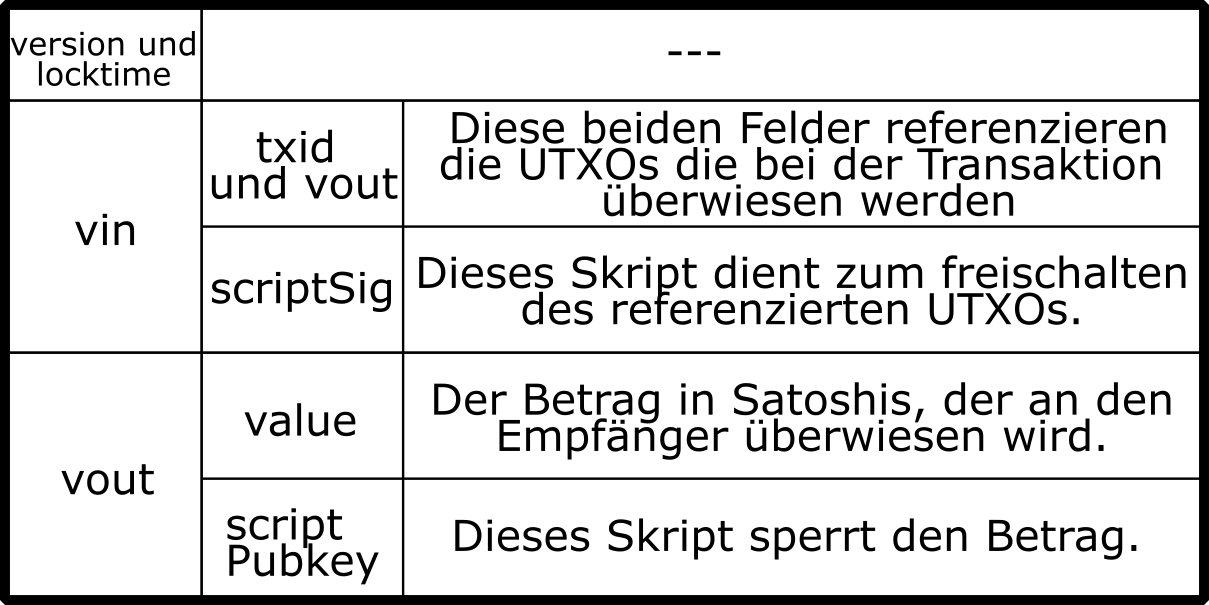
\includegraphics[width=.8\textwidth]{grafiken/tableTransaction.png}
  \caption{Zeigt die für diese Arbeit relevanten Felder einer Transaktion.}
  \label{fig:transactionTable}
\end{figure}

\subsection{Aufbau und Funktionsweise von Transaktionen}

\Cref{fig:transactionTable} zeigt den Aufbau einer Transaktion. Das Feld \textit{vout} beschreibt die neuen UTXOs (eine Liste), die bei der Transaktion angelegt werden. Jeder dieser UTXOs hat einen Betrag und ein Skript, das zur Freischaltung des Betrags erfüllt werden muss. Das Skript ist in der Sprache \textit{Script} geschrieben. Mit einem solchen Skript werden Signaturen erzeugt und geprüft. In den meisten Fällen wird der UTXO mit dem \textit{Pay-to-Public-Key-Hash} \citep{bitcoinbook} Skript gesperrt. Das bedeutet, dass zum Entsperren eine Signatur über die Transaktion benötigt wird.  Im Feld \textit{vin} werden die Geldmittel spezifziert, die versendet werden. Dies passiert über die Referenz auf UTXOs, die in \textit{vout} Abschnitten von anderen Transaktionen stehen.

Auf diese Weise entsteht eine Verkettung von Transaktionen. Die UTXOs einer Transaktion dienen als Geldmittel für eine andere Transaktion, welche wieder neue UTXOs anlegt und wieder als Geldmittel verwendet werden können. Die UTXOs sind dabei unteilbar. Soll zum Beispiel eine Transaktion über 5 Bitcoin durchgeführt werden und es steht nur ein UTXO in Höhe von 10 Bitcoin zur Verfügung\footnote{Der Betrag eines UTXOs wird nur einmal im vout Feld einer Transaktion spezifiziert. Im vin ist der Betrag implizit über die Referenz auf den UTXO enthalten.}, so muss der Sender zwei UTXOs im vout Feld definieren. Einen für den Empfänger über 5 Bitcoin und einen für sich selbst als Wechselgeld.

Bei jeder Transaktion werden außerdem Gebühren durch den Sender definiert. Diese Gebühren sind nicht notwendig, allerdings beschleunigen sie die Verifikation der Transaktion und spielen eine wichtige Rolle beim Mining (\Cref{sec:mining}). Die Gebühren werden über die Differenz der vin und der vout Beträge implizit angegeben.

\subsection{Block}\label{sec:block}

Die im letzten Abschnitt beschriebenen Transaktionen werden in sogenannten Blöcken aggregiert, um innerhalb des Bitcoin-Netzwerks eine einheitliche Sicht (Konsens) darüber zu schaffen, welche UTXOs existieren und welche bereits ausgegeben wurden. Ein Block beginnt mit einigen Metadaten und dem \textit{Block Header}. Der Block Header enthält einige für das Mining und der Konsensfindung relevante Felder, welche im Folgenden erklärt werden.

\begin{figure}
  \centering
  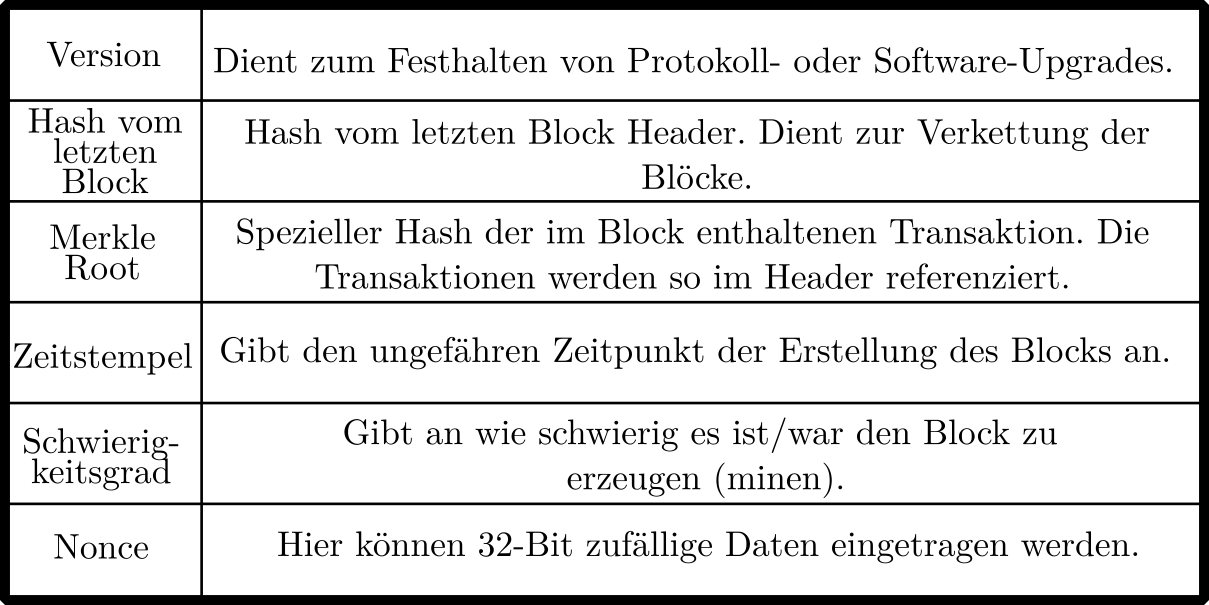
\includegraphics[width=.8\textwidth]{grafiken/tableBlock.png}
  \caption{Zeigt den Aufbau des Block Headers.}
  \label{fig:blockTable}
\end{figure}

\Cref{fig:blockTable} zeigt den Aufbau des Block Headers. Der Hash vom letzten Block (beziehungsweise vom letzten Block Header) ist eines der wichtigsten Elemente im Block. Er sorgt dafür, dass Blöcke miteinander verknüpft sind. Die Blöcke formen damit eine Kette von Blöcken, welche als Blockchain bezeichnet wird. Die Merkle Root ist eine Zusammenfassung der im Block enthaltenen Transaktionen \citep{bitcoinbook}. Sie stellt sicher, dass eine Veränderung der Transaktionen eine Veränderung des Headers zur Folge hat. Der Schwierigkeitsgrad und die Nonce werden bei der Erstellung (Mining) eines Blocks verwendet. Um einen gültigen Block zu erzeugen, muss der Hash des Headers kleiner sein als der Schwierigkeitsgrad (auch \textit{Difficulty Target} genannt), der im Header spezifiziert wird. Da das Ergebnis einer Hashfunktion nicht vorhergesagt werden kann, müssen verschiedene Header ausprobiert werden. Das Nonce Feld im Header dient zur Veränderung des Headers und damit zur Veränderung des Hashwerts. Andere Felder dürfen nicht verändert werden, da der Header sonst nicht mehr gültig ist. Um das Target zu unterschreiten, muss Rechenleistung aufgebracht werden (testen vieler verschiedener Nonce Werte). Dass diese Leistung tatsächlich erbracht wurde, kann mit einem einzelnen Durchlauf durch die Hashfunktion und anschließendem Vergleich mit dem \textit{Difficulty Target} verifiziert werden. Dieser Vorgang wird \textit{Proof-of-Work} genannt.

\subsection{Betrug in Bitcoin}\label{sec:betrug}

Mit den in \Cref{sec:transaktionen} besprochenen Mechanismen kann ein Empfänger von Bitcoins bestätigen, dass der Absender der tatsächliche Besitzer der Bitcoins ist. Der Empfänger kann die Signaturen verifizieren, um die Kette des Besitzes zurückzuverfolgen \citep{bitcoinPDF}. Es ist also nicht möglich Bitcoins zu kopieren oder zu erzeugen, da die Bitcoins bis zu ihrem Ursprung zurückverfolgt werden können. Die Transaktionen werden dafür in der Blockchain gespeichert (siehe \Cref{sec:block}). Dabei stellt sich die Frage, wie in einem verteilten System Einigkeit über den Zustand der Blockchain entstehen kann und wie diese gegen Veränderung geschützt wird. Wäre es möglich eine Transaktion im Nachhinein zu verändern, so könnte ein Käufer dieselben Bitcoins mehrfach ausgeben. In den nachfolgenden Abschnitten wird die Lösung dieses sogenannten \textit{Double-Spend-Problems} durch Mining und das Befolgen einiger Regeln durch jeden Netzwerkknoten beschrieben.


\section{Informationsverbreitung}\label{sec:informationsverbreitung}

In den folgenden beiden Abschnitten werden die Regeln beschrieben, mit denen Transaktionen und Blöcke vom Bitcoin-Netzwerk akzeptiert und verteilt werden. Das Netzwerk ist ein \textit{Peer-to-Peer Netzwerk}. Die Knoten in einem P2P Netzwerk sind gleichgestellt, jedoch nehmen sie im Bitcoin-Protokoll unterschiedliche Aufgaben wahr. Nachfolgend werden Knoten, die Routing Aufgaben übernehmen und eine komplette Kopie der Blockchain enthalten als \textit{Full Nodes} bezeichnet. Als Wallet werden Knoten bezeichnet, die lediglich die Schlüssel eines Nutzers verwalten und sich an Full Nodes wenden, um Zugriff auf die Blockchain zu erhalten. In \Cref{sec:mining} wird zusätzlich der Begriff \textit{Miner} für Knoten verwendet, die Mining durchführen. \Cref{fig:basicNetwork} zeigt einen Teil dieser Komponenten in einem einfachen Bitcoin-Netzwerk. 


\begin{figure}
  \centering
  \frame{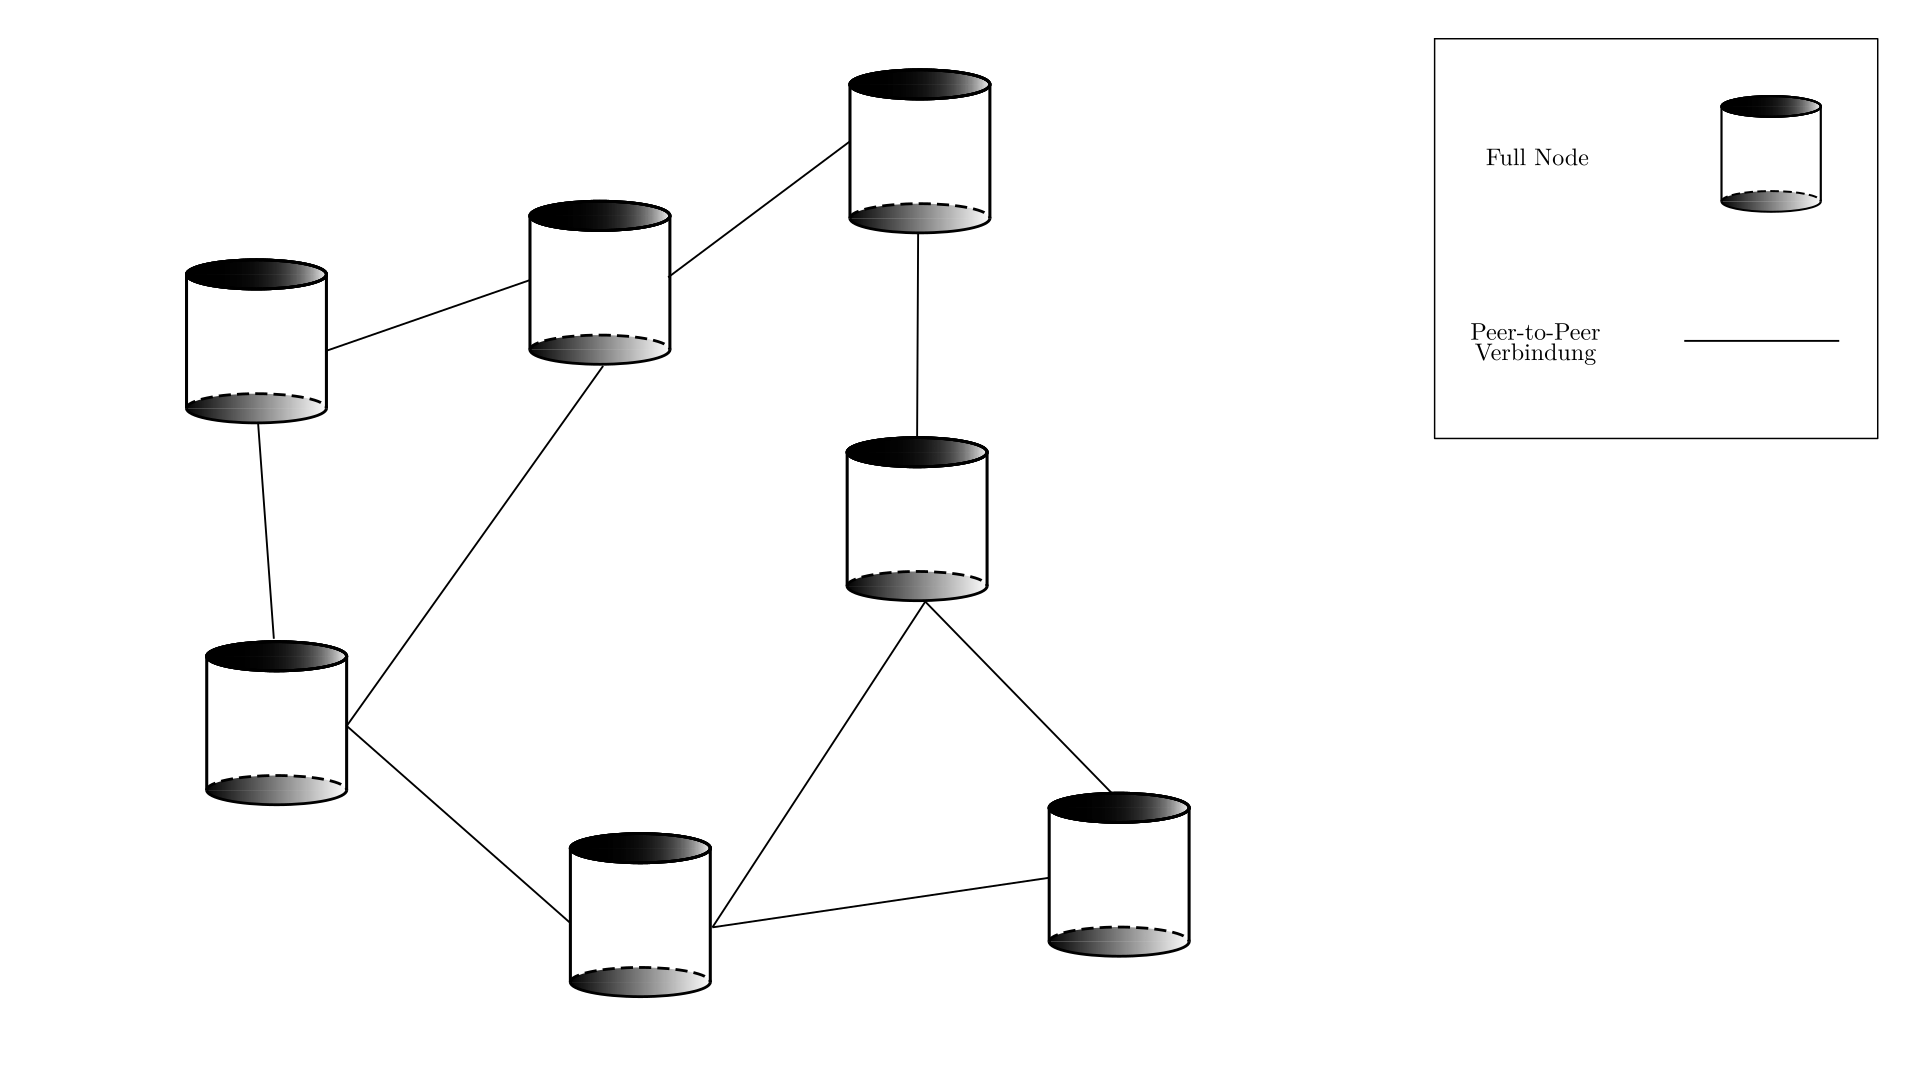
\includegraphics[width=.8\textwidth]{grafiken/network.png}}
  \caption{Der Aufbau eines einfachen Bitcoin-Netzwerks mit Peer-to-Peer Verbindungen und Full Nodes.}
  \label{fig:basicNetwork}
\end{figure}

\subsection{Verbreitung von Transaktionen}\label{sec:transaktionsverbreitung}

Eine Transaktion wird typischerweise in einem Wallet-Knoten erzeugt. Zum Beispiel wenn ein Nutzer einen anderen für einen Service oder ein Produkt bezahlen möchte. Die Transaktion wird entsprechend der in \Cref{sec:transaktionen} beschriebenen Struktur aufgebaut und anschließend über eine Full Node an das P2P Netzwerk übergeben. Beim Erhalt einer Transaktion werden dessen Struktur und Inhalt überprüft. Falls alle Kriterien erfüllt sind, wird die Transaktion an benachbarte Knoten weitergegeben und in den lokalen Speicher für unbestätigte Transaktionen übertragen (auch \textit{Memory Pool} oder \textit{Transaction Pool} genannt). In \Cref{fig:transactionPropagation} wird dieser Vorgang mit einer einzelnen Transaktion dargestellt. Die Transaktion wird in vereinfachter Form nur über die ID (txid) dargestellt, die normalerweise 256-Bit lang ist.

\begin{figure}
  \centering
  \frame{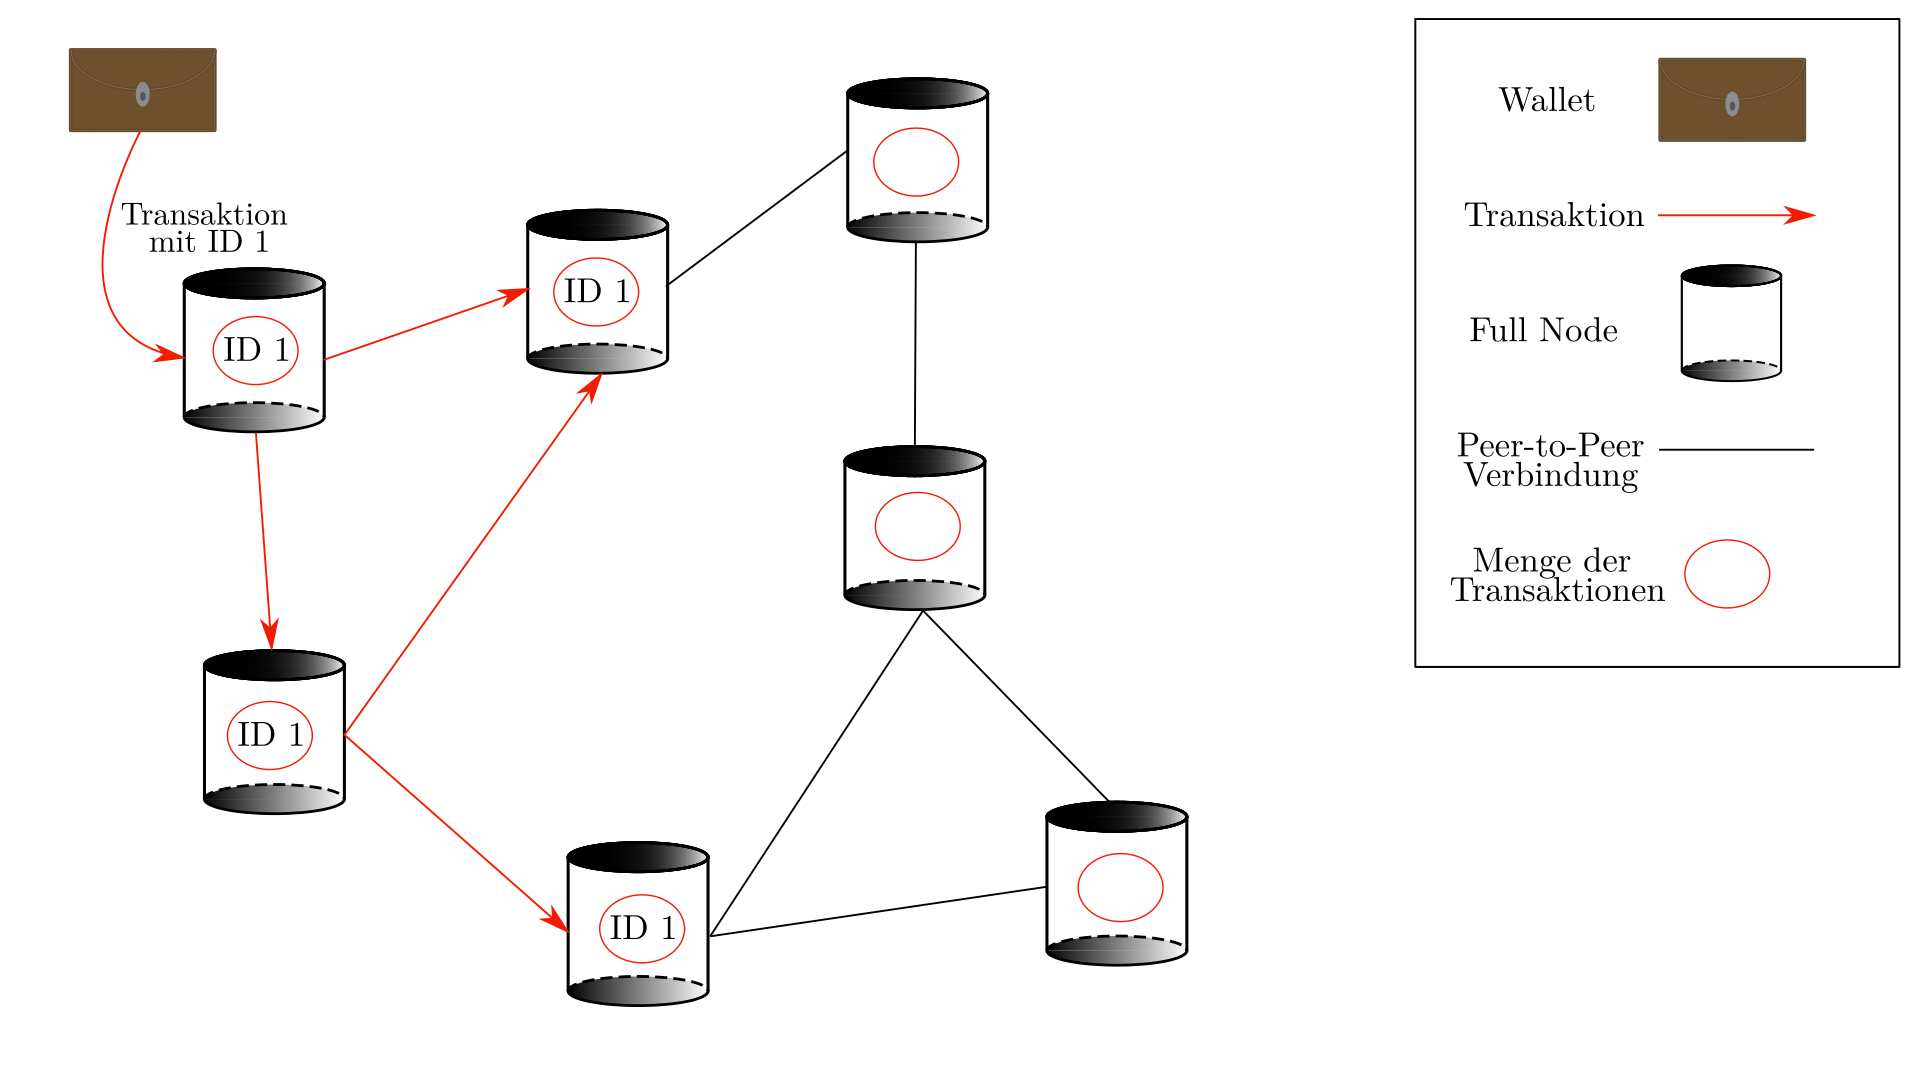
\includegraphics[width=.8\textwidth]{grafiken/transactionPropagation.png}}
  \caption{Die Verbreitung einer Transaktion im P2P Netzwerk. Nach der Überprüfung einer Transaktion wird diese im Memory Pool gespeichert und an benachbarte Knoten weitergeleitet.}
  \label{fig:transactionPropagation}
\end{figure}

Um zu bestätigen, dass eine Transaktion gültig ist, wird zunächst deren Aufbau auf Korrektheit überprüft. Danach werden einige formale Aspekte des Inhalts überprüft wie zum Beispiel ob die Maximallänge überschritten wurde oder die vin- und vout-Liste beide mindestens ein Element haben. Weitere wichtige Kriterien\footnote{Es gibt weitere Kriterien, die allerdings weniger relevant für das Verständnis des Minings und der Konsensfindung sind. Diese Regeln sind in \citep{bitcoinbook} oder im Bitcoin Source Code \citep{bitcoincore} aufgelistet.} sind:

\begin{itemize}

\item Die txids von allen vin Elementen müssen im Transaction Pool oder in einem Block der Blockchain\footnote{Für schnelleren Zugriff werden diese im UTXO Set abgespeichert.} enthalten sein. Falls keine passende Transaktion für eines der Elemente gefunden wird, wird die Transaktion dem \textit{Orphan Transaction Pool} hinzugefügt.

\item Keiner der Inputs (vin Elemente) darf in einer anderen Transaktion als Input vorkommen, da er sonst bereits ausgegeben wurde. Das gilt auch für Transaktionen mit dem gleichen Input im Orphan Transaction Pool.

\item Die Skripte zum Sperren und Entsperren für jedes Input-Output-Paar müssen ein gültiges Ergebnis liefern.

\end{itemize}

Bei Verletzung einer der oben genannten Regeln wird diese Transaktion verworfen und nicht im Netzwerk verbreitet. Alle ehrlichen Full Nodes verhindern somit die Verbreitung von falschen oder betrügerischen Transaktionen. Es werden zum Beispiel Transaktionen aussortiert, deren Ersteller nicht Besitzer der UTXOs ist oder wenn eine Transaktion versucht, einen UTXO zweimal auszugeben. Durch diese einfachen Regeln entsteht damit Konsens im Netzwerk, welche Transaktionen gültig sind und welche nicht. Allerdings können doppelt ausgegebene UTXOs nur mithilfe der Blockchain aussortiert werden. Im nächsten Abschnitt wird eine weitere Menge von Regeln beschrieben, die im Netzwerk Konsens über den Zustand der Blockchain herstellen.

\subsection{Verbreitung von Blöcken und Aufbauen der Blockchains}\label{sec:blockverbreitung}

Nachdem ein Block von einem Mining Knoten erstellt wurde (siehe \Cref{sec:mining}), wird dieser an das Netzwerk übergeben. Ähnlich wie bei der Verbreitung von Transaktionen wird eine Menge von Regeln für jeden Block überprüft und im Falle einer Regelverletzung verworfen. Der Block muss die in \Cref{sec:block} beschriebene Struktur aufweisen. Außerdem muss der Hash des Headers kleiner sein als das angegebene \textit{Difficulty Target} und alle enthaltenen Transaktionen müssen die in \Cref{sec:transaktionsverbreitung} aufgeführten Regeln einhalten. Durch diese Regeln wird sichergestellt, dass keiner der Miner betrügt. Versucht ein Miner zum Beispiel falsche Transaktionen in einen Block einzubauen, wird der Block vom Netzwerk abgelehnt und nicht weiter verbreitet.

Wenn eine Full Node einen Block erhält, der die Regeln einhält, wird er versuchen diesen an die Blockchain anzuhängen. Dafür muss der Knoten herausfinden, welcher Block in der Blockchain der Vorgänger des neuen Blocks ist. Das Headerfeld Hash vom letzten Block wird dafür mit den letzten Blöcken der Blockchain verglichen. Dabei kann es zu drei Fällen kommen (siehe auch \Cref{fig:blockchainTypes}):

\begin{itemize}

\item Der passende Block ist das Ende (der neueste Block) der bestehenden Blockchain. Der Block wird an diese Blockchain, die auch \textit{Main Chain} genannt wird, angehängt.

\item Der passende Block ist nicht das Ende der Blockchain, sondern ein älterer Block, also ein Block, auf dessen Basis bereits neuere Blöcke erzeugt wurden. Auch dieser Fall ist für das Bitcoin-Protokoll normal, der Block wird an den alten Block angehängt und bildet eine sogenannte \textit{Secondary Chain}.

\item Der passende Block konnte nicht gefunden werden. Der Block wird im sogenannten Orphan Block Pool gespeichert bis der Elternblock empfangen wird und beide der Blockchain hinzugefügt werden können.

\end{itemize}

\begin{figure}
  \centering
  \frame{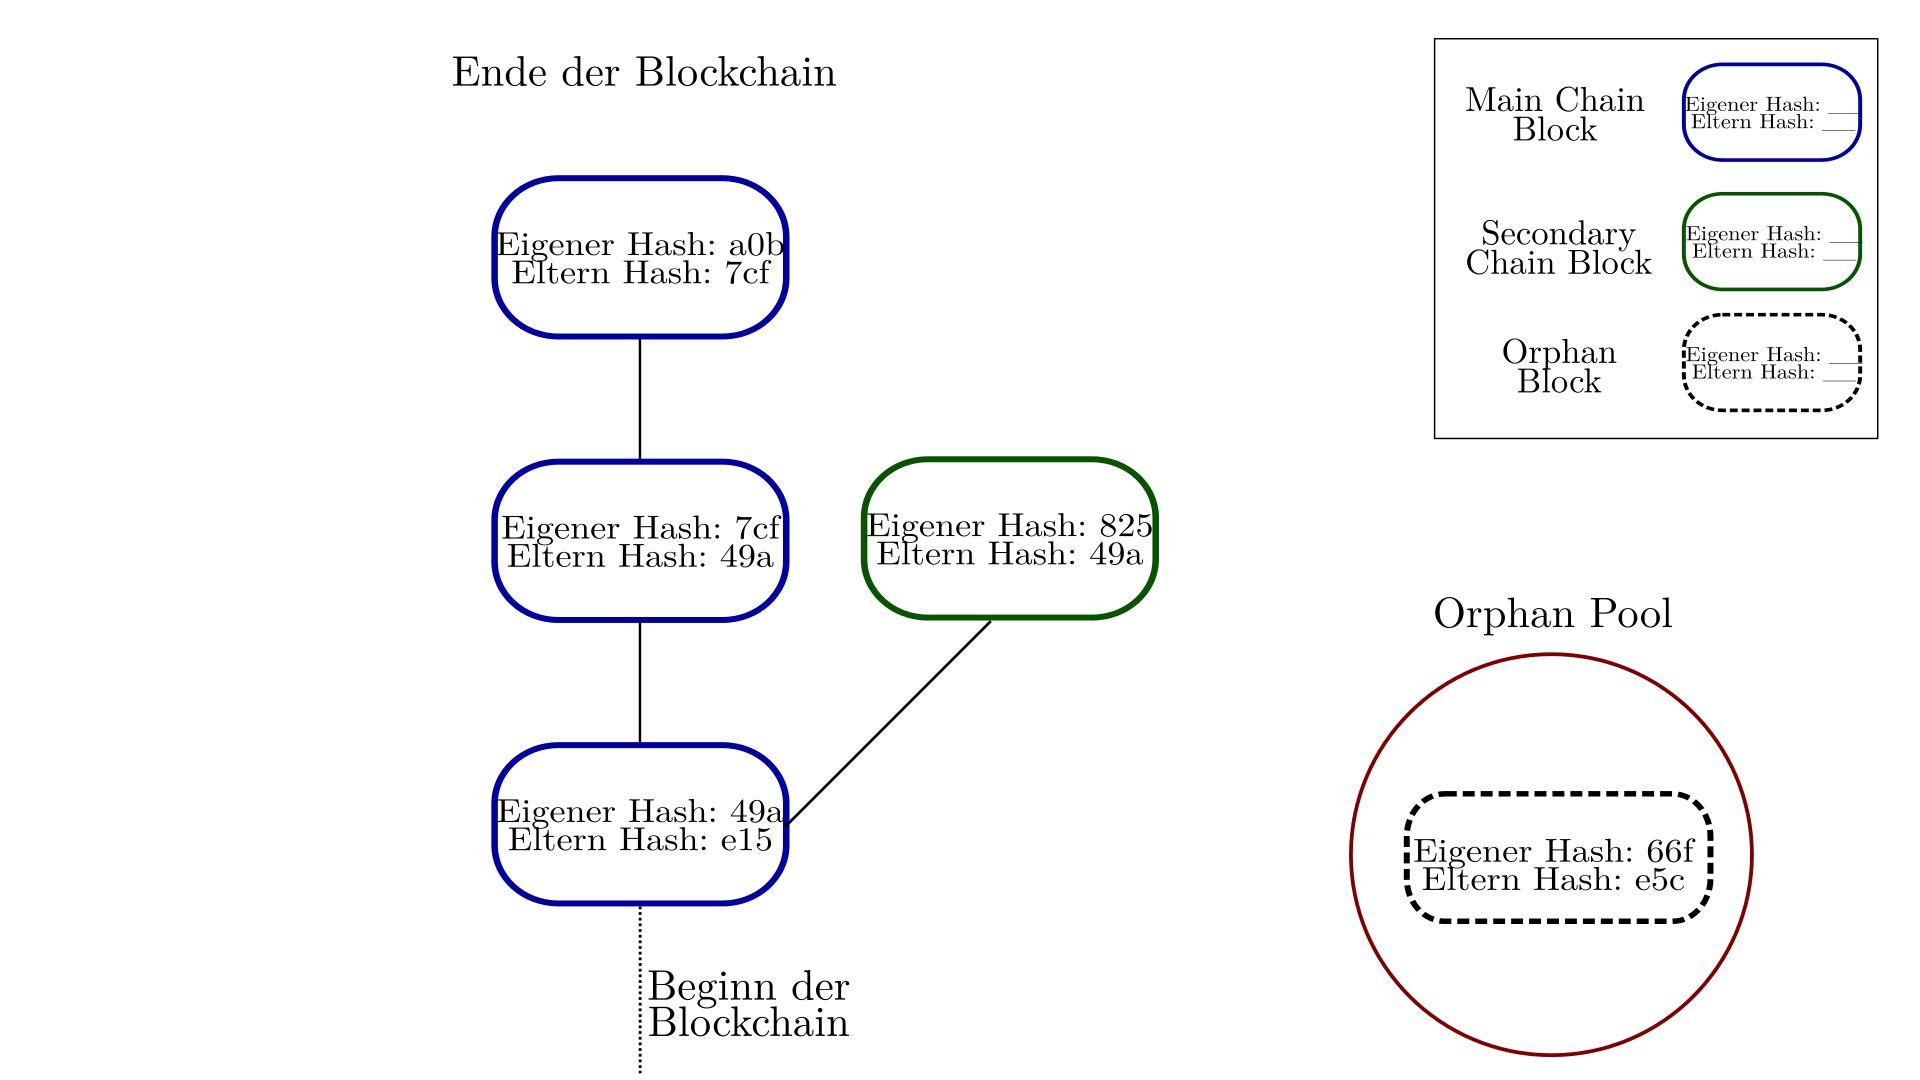
\includegraphics[width=.8\textwidth]{grafiken/blockchainTypes.png}}
  \caption{Die verschiedenen Typen von Blockchains: Main Chain, Secondary Chain und Orphan Pool.}
  \label{fig:blockchainTypes}
\end{figure}

In allen der aufgeführten Fälle wird der Block an benachbarte Knoten weitergeleitet. Falls zwei gültige Blöcke etwa zum gleichen Zeitpunkt\footnote{Tatsächlich ist dieser Zeitraum relativ groß. Solange ein Block noch nicht im gesamten Netzwerk verbreitet wurde, arbeitet ein Teil der Miner noch an der Suche nach dem alten Block (siehe \Cref{sec:mining}). Bis zur Verbreitung des Blocks im gesamten Netzwerk kann es zu 'gleichzeitigen' Einspeisung von Blöcken kommen.} ins Netzwerk eingespeist werden, kann es zu einem sogenannten Blockchain Fork kommen. Ein Teil des Netzwerks empfängt beispielsweise Block A zuerst und der andere Teil empfängt Block B zuerst. Letztendlich erhält jede Full Node beide Blöcke. Ein Teil des Netzwerks hat dann Block A als neuestes Main Chain Element und Block B als Secondary Chain Element eingetragen. Die anderen Knoten, die Block B zuerst erhalten haben, haben die Main und Secondary Chain exakt umgekehrt aufgebaut. Dieser Konflikt ist üblich und wird durch den nächsten Block, der ins Netzwerk eingespeist wird, gelöst. Basiert dieser neue Block auf Block A, dann werden alle Knoten die längere der beiden Ketten auswählen. Die längste Kette entspricht der Kette, in die die meiste Arbeit investiert wurde (\textit{Proof of Work}), da jeder Block etwa der gleichen Menge Arbeit entspricht.

\section{Mining}\label{sec:mining}

Der Begriff Mining lässt vermuten, dass das Mining primär für die Generierung neuer Bitcoins genutzt wird. Tatsächlich ist die Generierung neuer Bitcoins nur eine Belohnung neben den Gebühren für Miner. Dadurch werden Miner für ihre Suche nach einem neuen Block und die damit verbundene Arbeit belohnt. Für das Bitcoin-Protokoll dient das Mining hauptsächlich der Validierung und Aufzeichnung der Transaktionen auf der Blockchain. Durch die Aufzeichnung auf\todo{"auf" oder "in" hier} der Blockchain wird das sogenannte \textit{Double-Spend-Problem} gelöst (siehe \Cref{sec:betrug}).

Beim Mining werden Transaktionen in Blöcke zusammengefasst. Dafür benötigt ein Miner Zugriff auf den Transaction Pool einer Full Node. Ein Teil der im Pool enthaltenen Transaktionen wird für den nächsten Block ausgewählt. Die Auswahl wird dabei über die Größe des Blocks und die enthaltenen Gebühren getroffen. Der Block darf die maximale Blockgröße nicht überschreiten und der Miner bevorzugt Transaktionen mit hohen Gebühren. Zusätzlich wird die sogenannte Coinbasetransaktion als erste Transaktion in den Block eingefügt. Die Coinbasetransaktion enthält die Gebühren und die generierten Bitcoins, welche auf eine private Adresse überschrieben werden. Anschließend müssen alle Header Felder entsprechend der Definition gesetzt werden und der \textit{Proof-of-Work}-Algorithmus wird ausgeführt (siehe \Cref{sec:block}). Findet ein Miner einen Block oder empfängt ein Miner den Block, den ein anderer Miner gefunden hat, beginnt der Miner die Arbeit am nächsten Block. Nur der Miner, der den Block gefunden hat, erhält die volle Belohnung. Es handelt sich beim Mining also um einen \textit{Wettbewerb zwischen den Minern}\footnote{Oft arbeiten Miner in einem Mining Pool an der gemeinsamen Lösung des Problems und teilen die Gewinne entsprechend der zur Verfügung gestellten Rechenleistung auf.}.

Die Länge des Intervalls, in dem neue Blöcke der Blockchain hinzugefügt werden, soll konstant bei circa 10 Minuten liegen. Dabei handelt es sich um einen Kompromiss zwischen der schnellen Validierung von Transaktionen und der Verhinderung von Blockchain Forks. Um dieses Intervall sicherzustellen, wird die Zeit gesteuert, die ein Miner benötigt, um einen gültigen Block zu erzeugen. Durch den technologischen Fortschritt und die steigende oder sinkende Anzahl von Minern im Bitcoin-Netzwerk verändert sich die insgesamt zur Verfügung gestellte Rechenleistung (auch \textit{Hashing Power} genannt). Entsprechend wird die benötigte Zeit zum Minen eines Blocks größer oder kleiner. Um den zuvor beschriebenen Kompromiss zu gewährleisten, muss der Schwierigkeitsgrad des Minings kontinuierlich an die Rechenleistung angepasst werden. Hierfür wird in jeder Full Node alle 2016 Blöcke der Schwierigkeitsgrad angepasst. Dafür wird die tatsächlich benötigte Zeit für das Mining der letzten 2016 Blöcke mit der gewünschten Zeit (20160 Minuten) verglichen. Ist die benötige Zeit kleiner/größer, wird der Schwierigkeitsgrad erhöht/gesenkt.

\section{Konsens und Sicherheit}\label{sec:konsens}

Um zu verstehen warum, die in den letzten Abschnitten erläuterten Verfahren notwendig sind, lohnt sich eine erneute Betrachtung der grundlegenden Ideen von Bitcoin. Bitcoin ist eine dezentralisierte digitale Währung, die ohne eine zentrale Autorität auskommen soll. Das Mining dient dabei der Validierung von Transaktionen und ist damit essentiell für die Sicherheit von Bitcoin. Diese Validierung beziehungsweise das Mining muss dabei ebenfalls dezentralisiert ausgeführt werden. Das Mining ist dabei ein möglicher Angriffspunkt, da jeder daran teilnehmen und Transaktionen rückgängig machen kann. Bitcoin nutzt das Proof-of-Work-Verfahren, um es Angreifern möglichst schwer zu machen, solche Änderung durchzuführen.

Durch den Schwierigkeitsgrad (die Erstellung eines Blocks benötigt ca. 10 Minuten) und die Verkettung von Blöcken (siehe \Cref{sec:block}) muss ein Angreifer viel Arbeit aufwenden, um die Blockchain zu verändern. Verändert ein Angreifer zum Beispiel den vorletzten Block in der Blockchain, so muss er auch den letzten Block neu berechnen, da das Netzwerk nur die längste Kette akzeptiert, also die Kette, in der die meiste Arbeit (Proof-of-Work) steckt. Die Wahrscheinlichkeit, dass der Angreifer aufholt, sinkt exponentiell unter der Voraussetzung, dass die ehrlichen Miner mehr Hashing Power besitzen \citep{bitcoinPDF}. Damit ist es dem Angreifer nicht mehr möglich, alte Blöcke der Blockchain zu verändern, da der Rechenaufwand zu groß wird.

Der Schlüssel zur Sicherheit von Bitcoin ist also die Hashing Power der ehrlichen Miner immer größer zu halten als die Hashing Power eines Angreifers. Im Idealfall würde jeder verfügbare Rechner nur mit dem Mining von Bitcoin beschäftigt sein. Ein Angreifer kann damit unmöglich mehr Rechenleistung erhalten. Um möglichst nahe an diesen Idealfall zu kommen, muss ein Anreiz geschaffen werden, ehrliches Mining zu betreiben. Dieser Anreiz ist die in Cref{sec:mining} erwähnte Belohnung. Sie sollte größer sein als die aufzuwendenden Energiekosten und den Gewinn, den ein gelungener Angriff mit sich bringt. Durch den Wettbewerb zwischen Minern (siehe \Cref{sec:mining}) wird dieser Effekt noch verstärkt. Würde die Belohnung an alle beteiligten Miner gleichmäßig ausgezahlt, so würde es keinen Anreiz geben, die eigene Rechenleistung zu erhöhen. Durch den Wettkampf zwischen den ehrlichen Minern entsteht ein Wettlauf um mehr Rechenleistung, bei der ein Angreifer ebenfalls mithalten muss.

In \Cref{sec:blockverbreitung} wird beschrieben, wie jeder Knoten im Netzwerk den längsten Block auswählt. Die längste Kette bedeutet durch das Proof-of-Work-Verfahren auch, dass die Kette durch die größte Menge Hashing Power erstellt wurde. Die Annahme dabei ist, dass die größte Menge Hashing Power durch das Belohnungsverfahren immer auf der Seite der ehrlichen Miner liegt. Auf diese Weise entsteht im Netzwerk Konsens über den aktuell gültigen Stand der Blockchain und somit darüber, welche Geldmittel bereits ausgegeben wurden und welche nicht. Es kann dabei, wie in \Cref{sec:blockverbreitung} gezeigt, zu temporären Blockchain Forks kommen. Die Ursache hierfür könnte zum Beispiel ein Betrugsversuch sein oder auch gleichzeitig erstellte Blöcke. Im Falle eines Betrugsversuchs gelingt dieser nur, wenn wenige Blöcke (1-2) geändert werden müssen oder wenn die unehrliche Hashing Power über einen längeren Zeitraum größer ist als die Menge der ehrlichen Hashing Power.

\section{Zusammenfassung}\label{sec:Zusammenfassung}

Die Miner in Bitcoin sind essenzieller Bestandteil, um die Blockchain aufzubauen und damit das \textit{Double-Spend-Problem} zu lösen. Jeder ehrliche Miner stimmt mit seiner Rechenleistung für den korrekten Aufbau der Blockchain im Gegensatz zu anderen verteilten Systemen, bei denen pro IP-Adresse eine Stimme abgegeben wird. Der Mehrheitsentscheid ändert sich also von einem \textit{Wer besitzt die Meisten IPs?}-System hin zu einem \textit{Wer besitzt die größte Rechenleistung?}-System. Wer also die meiste Energie aufwenden kann, besitzt die Kontrolle über die Blockchain. Auf diese Weise wird das Bitcoin-Netzwerk weniger anfällig gegenüber Angriffen, da es für einen Angreifer schwieriger ist, eine große Menge Rechenleistung aufzubringen als eine große Menge IP-Adressen. Durch eine unabhängige Prüfung aller Blöcke und die Auswahl der längsten Kette wird Konsens im Netzwerk zwischen allen ehrlich agierenden Full Nodes hergestellt.

In Bitcoin wird also Sicherheit durch hohen Energieverbrauch (Mining) hergestellt. Dass der meiste Energieverbrauch auf der ehrlichen Seite liegt, wird durch die Belohnungen beim Mining sichergestellt. Allerdings ist die Rentabilität des Minings von äußeren Faktoren bestimmt. Dazu gehört der Wert (in konventionellen Währungen) von Bitcoin, Elektrizitätskosten, Hardwarekosten und die Menge der Bitcoin Nutzer bzw. die Höhe der Gebühren, die bei einer Transaktion anfallen. Die Sicherheit von Bitcoin basiert also auf äußeren Faktoren, auf die das Bitcoin-Netzwerk selbst keinen Einfluss hat. Außerdem sind die Schäden für die Umwelt von Bitcoin nicht vernachlässigbar. Würde Bitcoin global und als einzige Währung eingesetzt werden, würden die globalen CO\textsubscript{2}-Emissionen um 2,1 \% ansteigen. Dabei handelt es sich nur um Emissionen durch die Nutzung von Elektrizität. Der Wert läge noch höher, wenn Emissionen durch Kommunikationsinfrastruktur und Emissionen bei der Herstellung benötigter Hardware ebenfalls betrachtet werden. Demgegenüber sind die Emissionen eines vergleichbaren, global agierenden konventionellen Währungssystems vernachlässigbar \citep{Becker2013}. 

Das \textit{Proof-of-Work}-System eignet sich also, um das \textit{Double-Spend-Problem} zu lösen unter der Bedingung, dass die äußeren Faktoren stabil bleiben. Werden mit Bitcoin große Beträge überwiesen, sollte zudem gewartet werden, bis die Transaktion durch einige zusätzliche Blöcke (circa 6 Blöcke) bestätigt wurde, da dies die Wahrscheinlichkeit einer Änderung gegen Null gehen lässt (siehe \Cref{sec:konsens}). Die Frage der Umweltverträglichkeit eines solchen Systems bleibt jedoch offen. Hierfür müssen im Falle einer flächendeckenden Übernahme eines Systems wie Bitcoin Lösungen für eine Reduktion des Energieverbrauchs gefunden werden. 

\renewcommand{\bibsection}{\section*{Referenzen}} % requried for natbib to have "References" printed and as section*, not chapter*
% Use natbib compatbile splncsnat style.
% It does provide all features of splncs03, but is developed in a clean way.
% Source: http://phaseportrait.blogspot.de/2011/02/natbib-compatible-bibtex-style-bst-file.html
\bibliographystyle{splncsnat}
\begingroup
  \ifluatex
    %try to activate if bibliography looks ugly
    %\sloppy
  \else
    \microtypecontext{expansion=sloppy}
  \fi
  \small % ensure correct font size for the bibliography
  \bibliography{miningAndConsensus}
\endgroup

% Enfore empty line after bibliography
\ \\
%
Alle Links wurden am 17. Februar 2021 das letzte Mal aufgerufen.
\end{document}
